%%%%%%%%%%%%%%%%%%%%%%%%% Dokument %%%%%%%%%%%%%%%%%%%%%%%%%
\usepackage[a4paper, top=2.5cm, left=1.5cm, right=1.5cm, bottom=2cm]{geometry}
\setlength{\parindent}{0pt}

\usepackage[utf8]{inputenc}
\usepackage[IL2]{fontenc}
%\usepackage[slovak]{babel}
%\usepackage{a4wide}
\usepackage{amsmath,amsfonts,amssymb}
\usepackage{comment}

\usepackage[ddmmyyyy]{datetime}
\renewcommand{\dateseparator}{.}

\usepackage{eurosym}

\usepackage{graphicx}   % obrazky
\usepackage{wrapfig}    % obrazky

\usepackage{caption}    % popisky
\usepackage{subcaption} % popisky

\usepackage{listings}   % python
\usepackage{color}      % python

\usepackage{array}      % column width
\usepackage{calc}       % pocitanie vo funkciach (vspace,...)

\usepackage[shellescape,latex]{gmp}     % metapost
\usepackage{hyperref}   % url

\usepackage{siunitx}    % stvorcek (QED)
\setlength{\fboxsep}{.5\fboxsep}

\usepackage{pgfplots}   % grafy
\usepackage{pgf}        % grafy
\pgfplotsset{compat=1.15}

\usepackage{tikz}       % kreslenie

\pagenumbering{gobble}
\usepackage[pages=some]{background}
\usepackage[thinlines]{easytable}

\backgroundsetup{
scale=1,
color=black,
opacity=1,
angle=0,
contents={%
  \put(-299,200){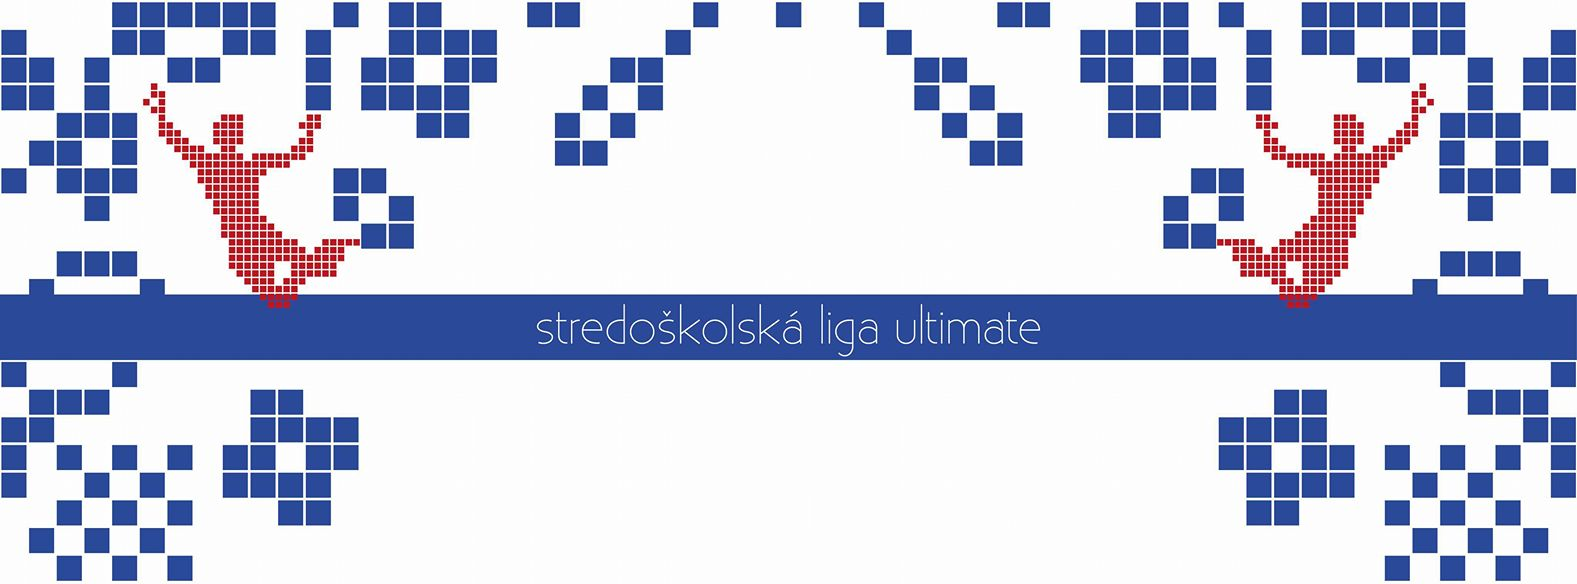
\includegraphics[width=\paperwidth]{images/title_image.jpg}}
  }%
}

\usepackage{stackengine}
\newcommand\funderline[1]{\underline{\stackengine{0pt}{\qquad}{#1}{O}{c}{F}{F}{L}}}
%%%%%%%%%%%%%%%%%%%%%%%%%%%%%%%%%%%%%%%%%%%%%%%%%%%%%%%%%%%%

%%%%%%%%%%%%%%%%%%%%%%%%% Ine makra %%%%%%%%%%%%%%%%%%%%%%%%
\def\obr#1#2{%
\begin{center}
\includegraphics[width=#1\textwidth]{#2}
\end{center}
}

\def\wrapobr#1#2#3#4#5#6{%
\begin{wrapfigure}[#1]{#2}{#3\textwidth}
\vspace{#4pt}
\begin{center}
\includegraphics[width=#5\textwidth]{images/#6}
\end{center}
\end{wrapfigure}
}

\def\wrapmpost#1#2#3#4#5#6{%
\begin{wrapfigure}[#1]{#2}{#3\textwidth}
\vspace{#4pt}
\centering
\resizebox{#5\textwidth}{!}{\input{images/#6}}
\end{wrapfigure}
}

\newcolumntype{C}[1]{>{\centering\let\newline\\\arraybackslash\hspace{0pt}}m{#1}}
\newcolumntype{L}[1]{>{\leftflushing\let\newline\\\arraybackslash\hspace{0pt}}m{#1}}
\newcolumntype{R}[1]{>{\rightflushing\let\newline\\\arraybackslash\hspace{0pt}}m{#1}}

\renewcommand{\arraystretch}{1.8}
%%%%%%%%%%%%%%%%%%%%%%%%%%%%%%%%%%%%%%%%%%%%%%%%%%%%%%%%%%%